\chapter{Application tests}

\section{Usability testing for the GUI front-end}
\label{test:canvas}
\begin{table}[h]
\begin{tabular}{|p{4.5cm}|p{4.5cm}|p{2cm}|p{2.5cm}|}
\hline
\textbf{Test} & \textbf{Pred. Result} & \textbf{Pass/ Fail} & \textbf{Comment}                        \\ \hline
Open menu    &   Menu is displayed on the left, canvas moves right. &  Pass          &    \\ \hline
Close menu    &   Menu hides to the left, canvas is pulled back in to fill page. &   Pass         &     \\ \hline
Resize window to mobile size    & Menu changes to mobile view, canvas still fills page.   & Pass           &     \\ \hline
Open mobile menu    & Menu displaying OLAN input, about and help pages listed.   &     Pass       &     \\ \hline
Open help page    &  Overlay appears from above, covers canvas with white box and text.  &       Pass     &     \\ \hline
Open about page    &  Overlay appears from above, covers canvas with white box and text.  &      Pass      &     \\ \hline
Close about page    &  Box fades away.  &      Pass      &     \\ \hline
Open sub-menu    &  Menu pulls in from left in side to cover current menu. Shows options of certain menu chosen.  &    Pass        &     \\ \hline
Click back on sub-menu    &  Sub-menu slides to left and reveals original top level menu.  &    Pass        &     \\ \hline
\end{tabular}
\caption{Usability test table for testing the GUI.}
\end{table}

\clearpage

\section{Test utility code for creating GUI before testing}
\label{test:utils}
\begin{figure}[h!]
\caption{RequireJS module for allowing test units to share methods providing them with GUI elements before tests. Tear down code removes the elements after each test.}
\begin{lstlisting}
define(function(){ 
	return {
		setUpAppend: function(toAppend) {
		            toAppend = "<div id='added'>" + toAppend + "</div>";
		            $('body').append(toAppend);
		},
        removeAppended: function(){
            $("#added").remove();
        }
	}
});
\end{lstlisting}
\end{figure}

\section{Test Unit code for converting JSON to manoeuvre instruction object}
\label{test:jsonmvoes}
\begin{figure}[h!]
\caption{JSUnit code created to test the capabilites of changing the JSON instructions into objects.}
\begin{lstlisting}
it(
    "Manouvres from JSON instructions should not be null",
    function(){
        ParseJson.init();
        expect( ParseJson.getManoeuvreArray() ).not.toBe(null);
    }
);
// There should be 27 OLAN manoeuvres
it(
    "Should be 27 OLAN manoeuvre objects in the JSON file",
    function(){
        ParseJson.init();
        expect( ParseJson.getManoeuvreArray().length ).toBe(27);
    }
);
// JSON instructions should come from intpu.
it(
    "JSON instructions should come from entering OLAN",
    function(){
        TestUtils.setUpAppend("<input id='input'/>");
        AnimationController.initControlEvents();
        ParseJson.init();
        $('#input').val('o');
        $('#input').keyup();
        expect( ParseJson.getManoeuvreArray().length ).toBe(27);
        TestUtils.removeAppended();
});
\end{lstlisting}
\end{figure}

\section{Test Unit code for checking lights and ground are created successfully}
\label{test:lights}
\begin{figure}[h!]
\caption{Checks if objects for both are created at runtime of the application.}
\begin{lstlisting}
// Load the terrain module and describe tests.
define(
    [
        "../../terrain"
    ],
    function( terrain ){
 
        // Describe the test suite for this module.
        describe(
            "The terrain module creates and returns both ground and ligting for the scene.",
            function(){
 
                // Check that terrain module creates a ground object, and returns it
                it(
                    "Ground should not be null",
                    function(){
 
                        expect( terrain.createGround() ).not.toBe(null);
                    }
                );

                // Check that the lighting object is successfully created and returned
                it(
                    "Lighting should not be null",
                    function(){
 
                        expect( terrain.setupLight() ).not.toBe(null);
                    }
                );
 
 
            }
        );
 
 
    }
);
\end{lstlisting}
\end{figure}

\clearpage

\section{Usability testing for cameras}
\label{test:cameras}
\begin{table}[h]
\begin{tabular}{|p{4.5cm}|p{4.5cm}|p{1cm}|p{4cm}|}
\hline
\textbf{Test} & \textbf{Pred. Result} & \textbf{Pass/ Fail} & \textbf{Comment}                        \\ \hline
Test drag mouse to rotate around canvas    &  Camera should rotate around the scene.  &     Fail       &  Changed after fail, due to camera rotation around the point(0,0,0). Changed now so that it rotates around current camera location.    \\ \hline
Scroll zoom in    &   Camera should focus in on the center of the canvas. &   Pass         &    \\ \hline
Scroll zoom out    &   Camera should see more of the canvas as mouse scrolls out. & Pass           &     \\ \hline
Left keyboard key to move left    &  Camera moves 10px to the left.  &   Pass         &     \\ \hline
Right keyboard key to move right    & Camera moves 10px to the right.   &    Pass        &     \\ \hline
Up keyboard key to move forward    &  Camera moves 10px forward its Z axis.  &   Pass         &     \\ \hline
Down keyboard key to move backwards    &  Camera moves 10px backwards its Z axis.  &  Pass          &     \\ \hline
Switch to onboard camera view   &  Camera changes to 0,0,0 looking ahead. &  Pass          &     \\ \hline
\end{tabular}
\caption{Tests various actions from the user to do with both cameras.}
\end{table}

\clearpage

\section{Test Unit code for animation controller getters and setters}
\label{test:animation}
\begin{figure}[h!]
\caption{Unit code checking information is set correctly, and if it can be changed at stored for various animation properties.}
\begin{lstlisting}
// Check that terrain module creates a ground object, and returns it
it(
    "Should be paused by default",
    function(){
        expect( animation.getIsPaused() ).toBe(true);
    }
);

// Check pause functionality works
it(
    "Should not be paused after clicking pause",
    function(){
        TestUtils.setUpAppend("<button id='pause'></button><input id='input'>");
        $('#input').val("o");

        animation.initControlEvents();
        $('#pause').click();
        expect( animation.getIsPaused() ).toBe(false);

        TestUtils.removeAppended();
    }
);

// check default speed
it(
    "Default speed of animation should be increments of 0.005",
    function(){
        expect( animation.getAnimationSpeed() ).toBe(0.005);
    }
);

// Check changing speed of animation works
it(
    "Speed should be 0.01 at maximum value of slider",
    function(){
        TestUtils.setUpAppend("<input id='speed' type='range' value='0.01' min='0.001' max='0.01' step='0.001' />");

        animation.initControlEvents();
        $('#speed').change();
        expect( animation.getAnimationSpeed() ).toBe(0.01);

        TestUtils.removeAppended();
    }
);
            
\end{lstlisting}
\end{figure}

\clearpage

\section{Test Unit code for checking import and export to JSON/ local storage functionality}
\label{test:save}
\begin{figure}[h!]
\caption{JSUnit code for checking flight paths export correctly to JSON and local storage, and check importing back works.}
\begin{lstlisting}
// Shoule be able to export and import from local storage
it(
    "Exporting to and then importing from localStorage should work",
    function(){
        ExportImportProjects.exportToLocalStorage("o a b o");
        expect( ExportImportProjects.importFromLocalStorage() ).toBe("o a b o");
    }
);

// Should export manoeuvres to JSON from the scenario
it(
    "Should be able to export to JSON",
    function(){
        var manoeuvres = "o a b o";
        var json = Utilities.convertManoeuvresToJSON(manoeuvres);
        expect( manoeuvres ).toBe(json["manoeuvres"]);
    }
);

// Should import manoeuvres from JSON to the scenario
it(
    "Should be able to import from JSON",
    function(){
        var manoeuvres = "o a b o";
        var json = Utilities.convertManoeuvresToJSON(manoeuvres);
        var result = Utilities.convertJSONToManoeuvres(json);
        expect( result ).toBe(manoeuvres);
    }
);

// Checks if local storage auto save switch correctly sets.
it(
    "Should be able to save change option of local storage on",
    function(){
        TestUtils.setUpAppend("<input id='autoSave' type='checkbox'>");
        AnimationController.initControlEvents();
        $('#autoSave').prop('checked', true);
        $('#autoSave').change();
        expect( ExportImportProjects.getAutoLoadLocal() ).toBe(true);
        $('#autoSave').prop('checked', false);
        $('#autoSave').change();
        TestUtils.removeAppended();
    }
);
\end{lstlisting}
\end{figure}

\section{Usability testing for GUI options}
\label{test:options}
\begin{table}[h]
\begin{tabular}{|p{4.5cm}|p{4.5cm}|p{2cm}|p{2.5cm}|}
\hline
\textbf{Test} & \textbf{Pred. Result} & \textbf{Pass/ Fail} & \textbf{Comment}                        \\ \hline
Type OLAN into input box to create figures    &  Loop should appear when 'o' is typed in, and movie-reel should show manouvre at bottom.  &            &     \\ \hline
Use dropdown in OLAN options to add a figure    &  Loop should be added to canvas when chosen from dropdown.  &     Pass       &     \\ \hline
Increase and decrease scale    &  Figures on canvas should become bigger or smaller depending on scale.  &       Pass     &     \\ \hline
Increase and decrease extrusion segments    &  Curves should become less and more smooth depending on extrusion.  &       Pass     &     \\ \hline
Increase and decrease radius    &  More sides to the figure should appear the higher the radius.  &     Pass       &     \\ \hline
Increase animation speed    &   Speed of flight should increase depending on slider of speed. &            &     \\ \hline
Turn switch on for auto repeat of animation    &  When on, when animating, should loop from beginning to end endlessly.  &       Pass     &     \\ \hline
Switch auto save on and close application, then re-open    &  When on, if application is closed and re-opened then routines should be added automatically. Vice versa.  &       Pass     &     \\ \hline
Export to JSON using button    &  JSON file begins to download on click.  &      Pass      &     \\ \hline
Import JSON file using file chooser  &  Routine should load up when selecting a file.  &      Pass      &     \\ \hline
\end{tabular}
\caption{Usability test table for user interface options, including OLAN entry box, OLAN dropdown, pyhsics options, animation options and exporting/ importing to JSON.}
\end{table}

\clearpage

\section{Usability testing providing parameters between OLAN}
\label{test:parameters}
\begin{table}[h]
\begin{tabular}{|p{4.5cm}|p{4.5cm}|p{2cm}|p{2.5cm}|}
\hline
\textbf{Test} & \textbf{Pred. Result} & \textbf{Pass/ Fail} & \textbf{Comment}                        \\ \hline
Enter empty parameters '()'    &  No change to start location of next manoeuvre should occur.  &     Pass       &     \\ \hline
Empty correct format paramaters '(10,10)'    &  Should move start of next manoeuvre 10 pixels up, 10 to the left.  &      Pass      &     \\ \hline
Enter parameters without space between OLAN    & The manouvre nor parameters will be placed on the canvas.   &        Pass    &     \\ \hline
Enter parameters with negative values '(-10,-10)'    &  Should move start of next manoeuvre 10 pixels down, 10 to the right.  &       Pass     &     \\ \hline
Enter parameters on a manoeuvre "o''"  &  Loop should be drawn with three times the length exit travel.  &        Fail    &   Parameter had np effect to the loops exit, and prevented the manouvre from being drawn.  \\ \hline
\end{tabular}
\caption{Usability test table showing results of typing in parameters alongside maneouvres.}
\end{table}

\clearpage

\section{User questionnaire}
\label{test:questionnaire}
\begin{figure}[h!]
    \caption{A google forms questionnaire created to allow users to give feedback about the application.}
    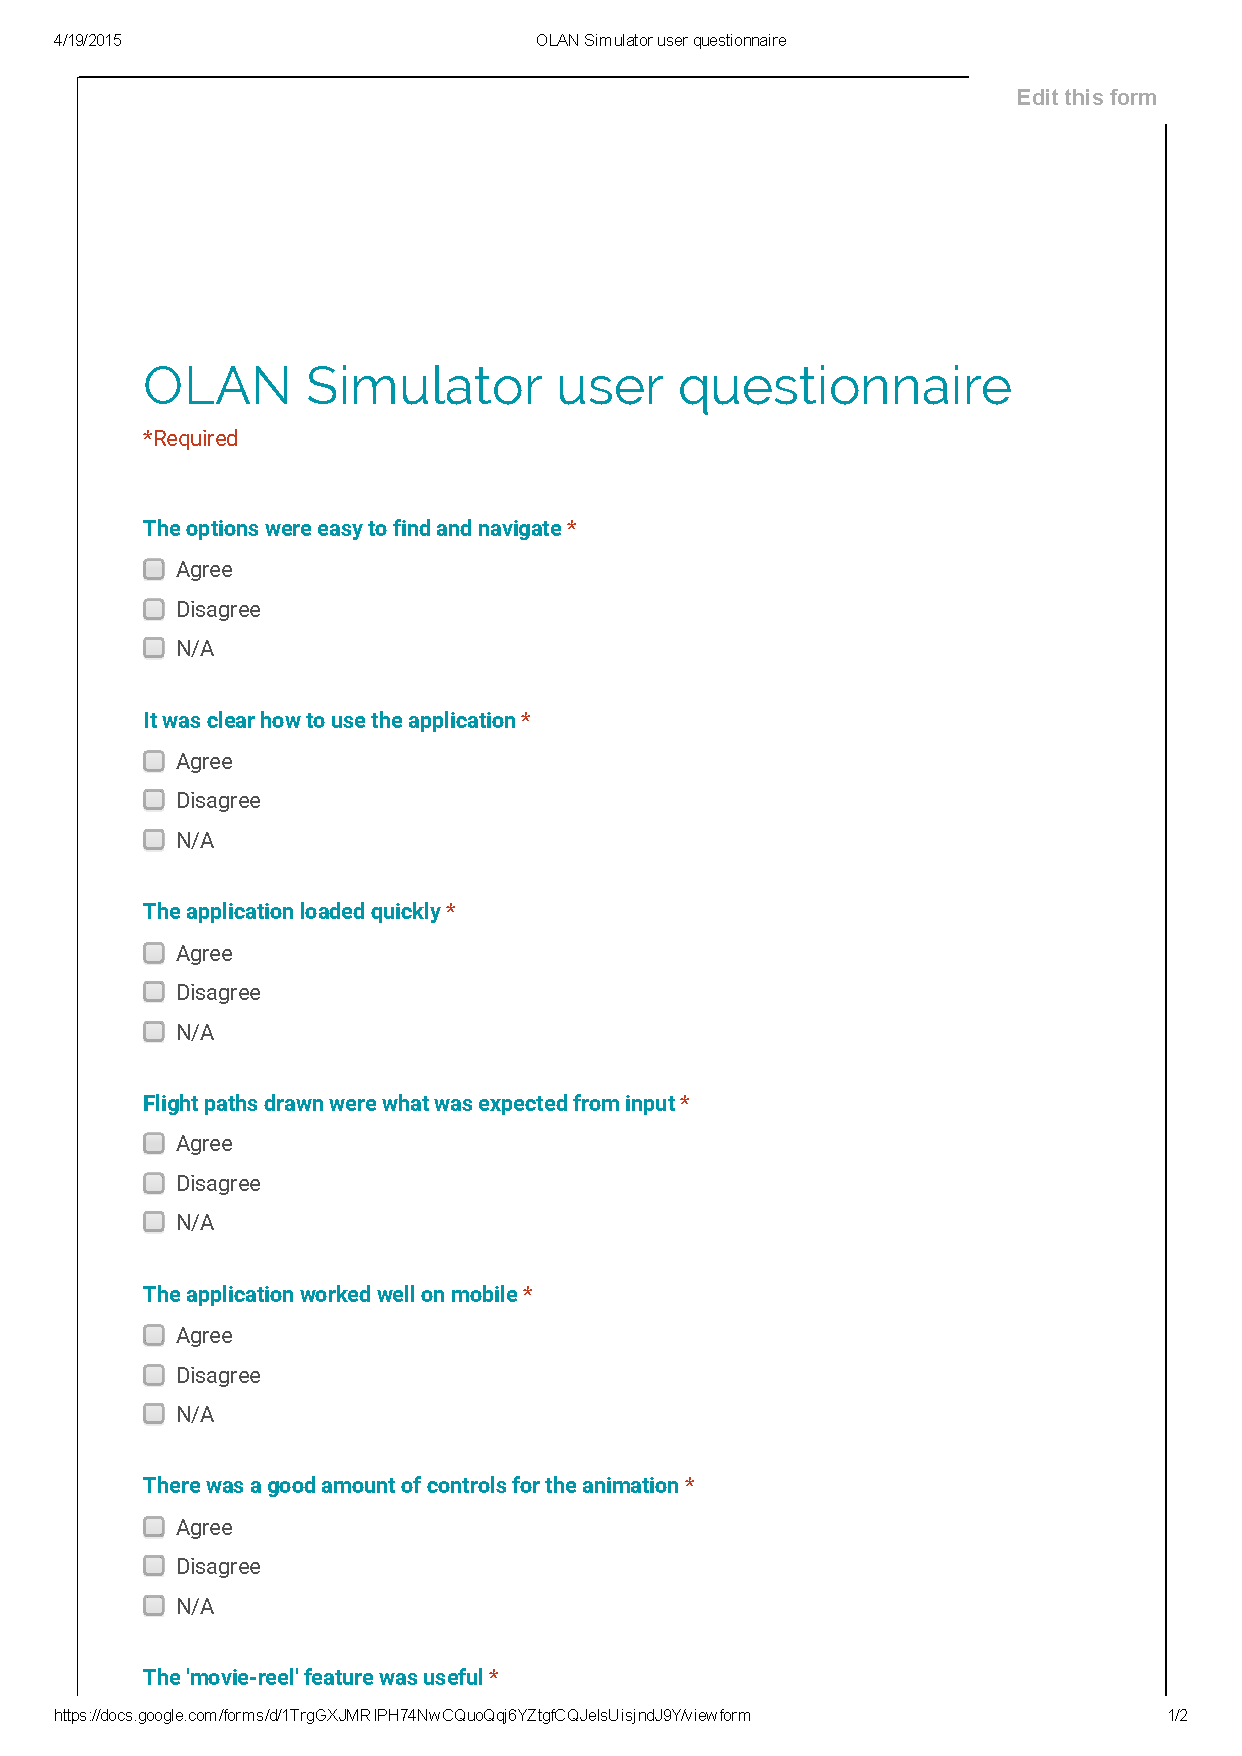
\includegraphics[width=15cm,height=18cm,page=1]{images/questionnaire.pdf}
\end{figure}

\begin{figure}[h!]
    \includegraphics[width=15cm,height=18cm,page=2]{images/questionnaire.pdf}
\end{figure}

\clearpage

\section{User questionnaire results}
\label{test:questionnaireResults}
\begin{figure}[h!]
    \caption{Statistics from the questionnaire results, showing percentages of answers and comments/ suggestions.}
    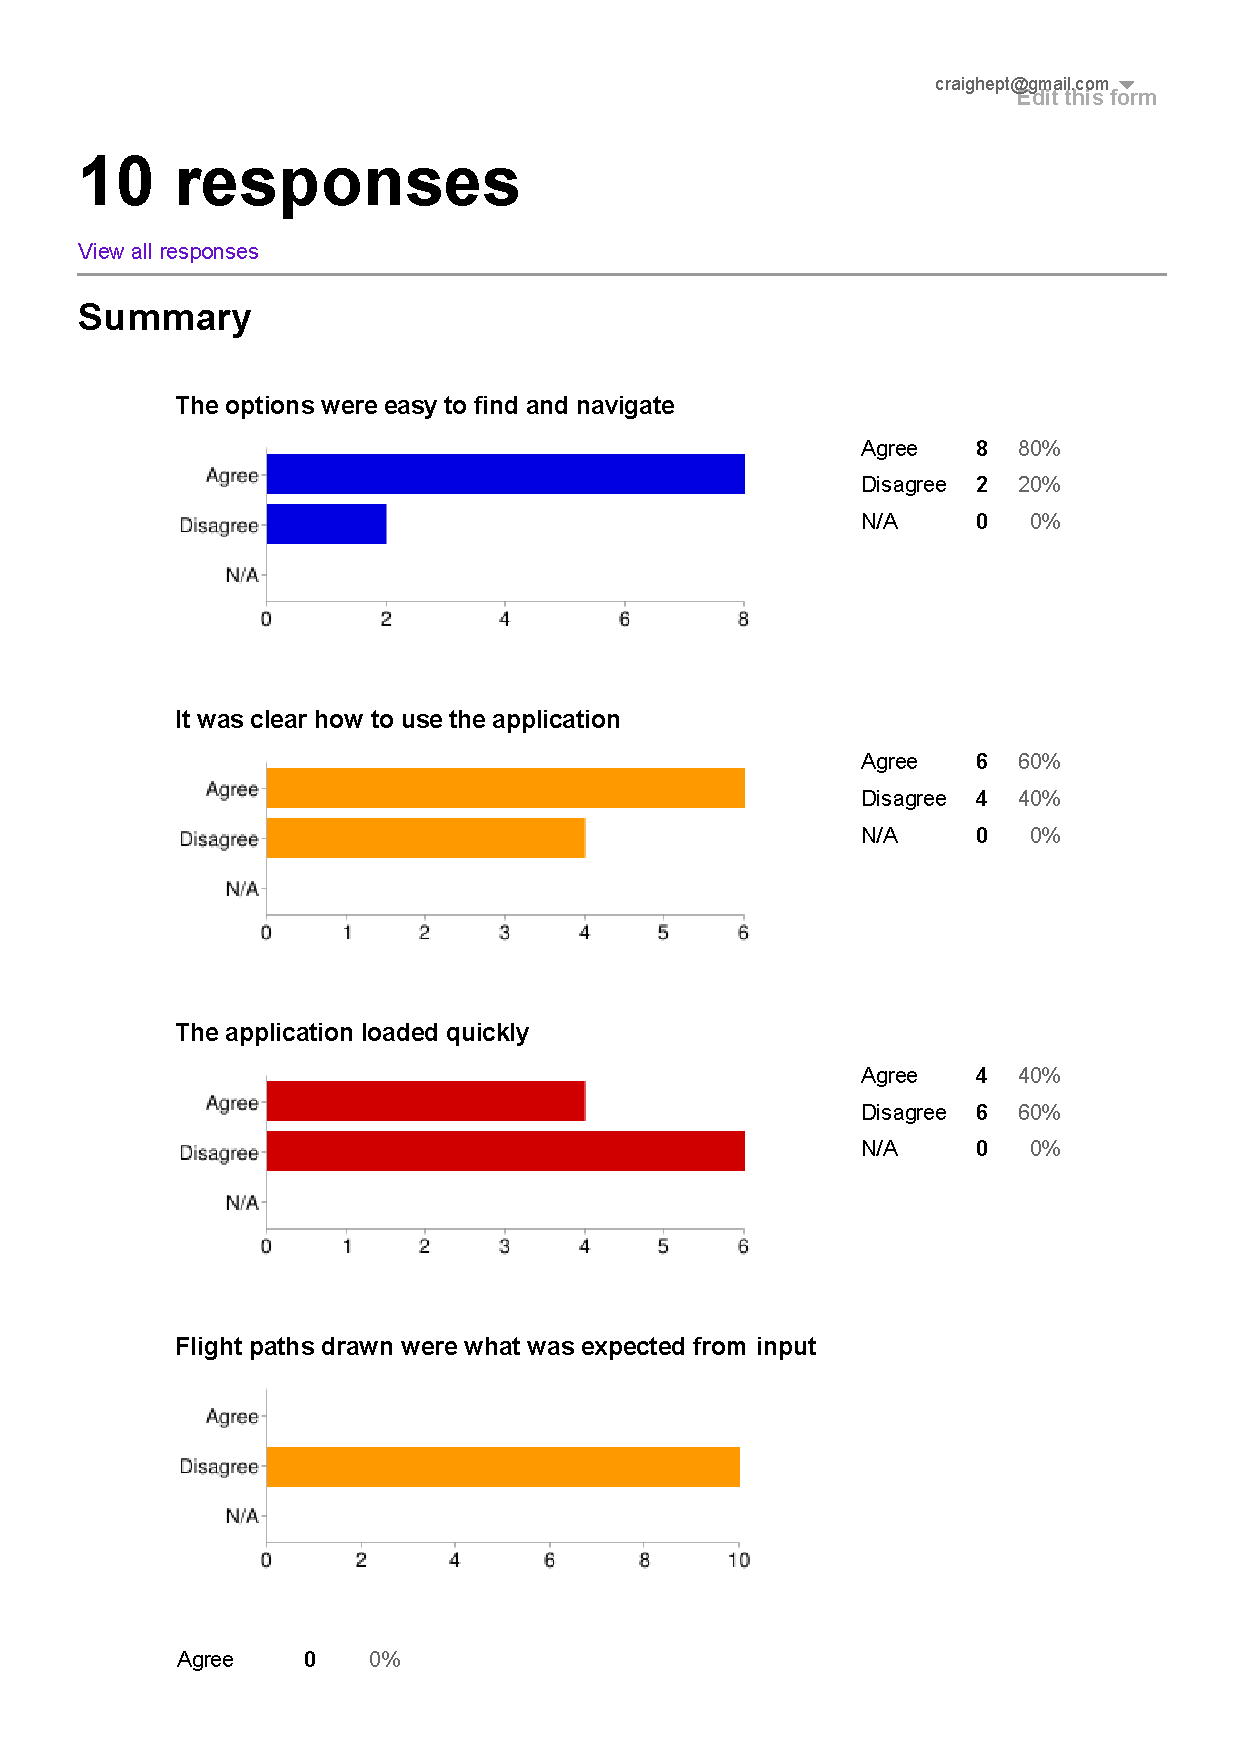
\includegraphics[width=15cm,height=18cm,page=1]{images/questionnaireResults.pdf}
\end{figure}

\begin{figure}[h!]
    \includegraphics[width=15cm,height=18cm,page=2]{images/questionnaireResults.pdf}
\end{figure}

\begin{figure}[h!]
    \includegraphics[width=15cm,height=18cm,page=3]{images/questionnaireResults.pdf}
\end{figure}